\documentclass[nonacm]{acmart}
\settopmatter{printfolios=true,printccs=true,printacmref=true}

%%
%% Bibliography and Citation Style
%%
\bibliographystyle{ACM-Reference-Format}
\citestyle{acmauthoryear}

\usepackage{mathtools}
\usepackage{amsmath}
\usepackage{cleveref}
\usepackage{bussproofs}
\usepackage{listings}

%%
%% Macros
%%
%%
%% Terms
%%
\newcommand{\lit}[1]{\ensuremath{\ulcorner #1 \urcorner}}
\newcommand{\cut}[2]{\ensuremath{\langle #1 \mid #2 \rangle}}
\newcommand{\done}{\ensuremath{\mathbf{done}}}
\newcommand{\ifz}[3]{\ensuremath{\mathbf{ifz}(#1, #2, #3)}}
\newcommand{\letin}[3]{\ensuremath{\mathbf{let}\ #1 = #2\ \mathbf{in}\ #3}}
\newcommand{\caseof}[2]{\ensuremath{\mathbf{case}\ #1\ \mathbf{of}\ \{ #2 \}}}
\newcommand{\case}[1]{\ensuremath{\mathbf{case}\ \{ #1 \}}}
\newcommand{\cocase}[1]{\ensuremath{\mathbf{cocase}\ \{ #1 \}}}
\newcommand{\goto}[2]{\ensuremath{\mathbf{goto}(#1; #2)}}
\newcommand{\lab}[2]{\ensuremath{\mathbf{label}\ #1\ \{#2 \}}}
\newcommand{\defi}[2]{\ensuremath{\mathbf{def}\ #1 \coloneq #2}}

%%
%% AxCut Terms
%%
\newcommand{\jump}[1]{\ensuremath{\mathbf{jump}\, #1}}
\newcommand{\invoke}[2]{\ensuremath{\mathbf{invoke}\, #1\, #2}}
\newcommand{\switch}[2]{\ensuremath{\mathbf{switch}\, #1\, #2}}
\newcommand{\substitute}[2]{\ensuremath{\mathbf{substitute}[#1];#2}}
\newcommand{\letac}[3]{\ensuremath{\mathbf{let}\, #1 = #2; #3}}
\newcommand{\new}[3]{\ensuremath{\mathbf{new}\, #1 = #2; #3}}
\newcommand{\bra}[1]{\ensuremath{\{ #1 \}}}
\newcommand{\ifzac}[3]{\ensuremath{\mathbf{ifz}(#1)\{ () \Rightarrow #2, () \Rightarrow #3 \}}}
\newcommand{\litac}[3]{\ensuremath{\mathbf{lit}[\lit{#1}]\{ #2 \Rightarrow #3 \}}}
\newcommand{\opac}[3]{\ensuremath{\odot(#1)\{ #2 \Rightarrow #3 \}}}

%%
%% Languages and Calculi
%%
\newcommand{\lambdamumu}{$\lambda\mu\tilde\mu$-calculus}
\newcommand{\surfacelang}{\textbf{Fun}}
\newcommand{\targetlang}{\textbf{Core}}
\newcommand{\machinelang}{\textbf{AxCut}}

%%
%% Types / Typing Rules / Typing Contexts
%%
\newcommand{\tyint}{\mathbf{Int}}
\newcommand{\wrap}[1]{:^{\text{\tiny#1}}}
\newcommand{\prd}{\wrap{prd}}
\newcommand{\cnt}{\wrap{cns}}
\newcommand{\wellformed}[1]{#1\ \textsc{Ok}}
\newcommand{\data}[2]{\mathbf{data}\, \mathtt{#1}\, \{ #2 \}}
\newcommand{\codata}[2]{\mathbf{codata}\, \mathtt{#1}\, \{ #2 \}}

%%
%% Evaluation / Reduction / Operational Semantics
%%
\newcommand{\reducesto}{\ensuremath{\triangleright}}


%%
%% Translations / Transfomations
%%
\newcommand{\focus}[1]{\ensuremath{\mathcal{F}(#1)}}
\newcommand{\name}[1]{\ensuremath{\mathcal{N}(#1)}}
\newcommand{\bind}[2]{\ensuremath{\mathsf{bind}(#1)[#2]}}
\newcommand{\redundancy}[1]{\ensuremath{\mathcal{R}(#1)}}
\newcommand{\fresh}[1]{\ensuremath{(#1\text{ fresh})}}
\newcommand{\translate}[1]{\ensuremath{\llbracket #1 \rrbracket}}
\newcommand{\translatestar}[2]{\ensuremath{\llbracket #1 \rrbracket_{#2}^{\ast}}}


\begin{document}
%%
%% Title information
%%
\title{Compiling with Sequent Calculus}
\subtitle{A unifying approach
for control effects and codata types}

%%
%% Keywords
%%
\keywords{Intermediate representations, continuations, codata types, control effects}

%%
%% CCS Classification
%%

\begin{CCSXML}
  <ccs2012>
     <concept>
         <concept_id>10003752.10003753.10003754.10003733</concept_id>
         <concept_desc>Theory of computation~Lambda calculus</concept_desc>
         <concept_significance>500</concept_significance>
         </concept>
     <concept>
         <concept_id>10011007.10011006.10011041</concept_id>
         <concept_desc>Software and its engineering~Compilers</concept_desc>
         <concept_significance>500</concept_significance>
         </concept>
     <concept>
         <concept_id>10011007.10011006.10011008.10011024.10011027</concept_id>
         <concept_desc>Software and its engineering~Control structures</concept_desc>
         <concept_significance>300</concept_significance>
         </concept>
   </ccs2012>
\end{CCSXML}

\ccsdesc[500]{Theory of computation~Lambda calculus}
\ccsdesc[500]{Software and its engineering~Compilers}
\ccsdesc[300]{Software and its engineering~Control structures}

%%
%% Author: David Binder
%%
\author{David Binder}
\orcid{0000-0003-1272-0972}
\affiliation{
  \department{Department of Computer Science}
  \institution{University of Tübingen}
  \city{Tübingen}
  \country{Germany}
}
\email{david.binder@uni-tuebingen.de}

%%
%% Author: Marco Tzschentke
%%
\author{Marco Tzschentke}
\orcid{0009-0004-8834-2984}
\affiliation{
  \department{Department of Computer Science}
  \institution{University of Tübingen}
  \city{Tübingen}
  \country{Germany}
}
\email{marco.tzschentke@uni-tuebingen.de}

%%
%% Author: Marius Müller
%%
\author{Marius Müller}
\orcid{0000-0002-0260-6298}
\affiliation{
  \department{Department of Computer Science}
  \institution{University of Tübingen}
  \city{Tübingen}
  \country{Germany}
}
\email{mari.mueller@uni-tuebingen.de}

%%
%% Author: Philipp Schuster
%%
\author{Philipp Schuster}
\orcid{0000-0001-8011-0506}
\affiliation{
  \department{Department of Computer Science}
  \institution{University of Tübingen}
  \city{Tübingen}
  \country{Germany}
}
\email{philipp.schuster@uni-tuebingen.de}

%%
%% Author: Jonathan Immanuel Brachthäuser
%%
\author{Jonathan Immanuel Brachthäuser}
\orcid{0000-0001-9128-0391}
\affiliation{
  \department{Department of Computer Science}
  \institution{University of Tübingen}
  \city{Tübingen}
  \country{Germany}
}
\email{jonathan.brachthaeuser@uni-tuebingen.de}

%%
%% Author: Klaus Ostermann
%%
\author{Klaus Ostermann}
\orcid{0000-0001-5294-5506}
\affiliation{
  \department{Department of Computer Science}
  \institution{University of Tübingen}
  \city{Tübingen}
  \country{Germany}
}
\email{klaus.ostermann@uni-tuebingen.de}

%%
%% Abstract
%%
\begin{abstract}
  Compiling a high-level functional programming language to machine code that can be executed efficiently on a modern machine is a complicated task, since we have to traverse many different levels of abstraction. This is particularly challenging if
  the language contains some form of control effects and/or a mix of different
  calling conventions, such as call-by-value data types and call-by-name codata types.
  In this paper we tell the complete story, starting from a simple functional programming language with control effects and both data and codata types, and ending up with Risc-V and x86-64 machine code.
  The novelty of our approach lies in the fact that we use the sequent calculus, and sequent calculus inspired languages, in specifying the intermediate stages of our compiler. In that sense, we view this work as a continuation, and generalization, of
  Andrew Appel's landmark work on Compiling with Continuations \cite{Appel1992compiling}.
\end{abstract}

\maketitle

%%
%% Section: Introduction
%%
\section{Introduction}
\label{sec:introduction}
Compiling a modern functional programming language like Haskell or OCaml to efficient machine code is a complicated affair, since we have to cross many different levels of abstraction in order to bridge the gap between high-level conveniences and low-level concerns.
In this paper we present such a complete compilation pipeline, starting with a surface language which supports different calling conventions, codata types and control effects, and ending up with machine code for Risc-V and X86-64.
More concretely, we show how to implement all of the following stages in the compiler pipeline:
\medskip

\begin{center}
  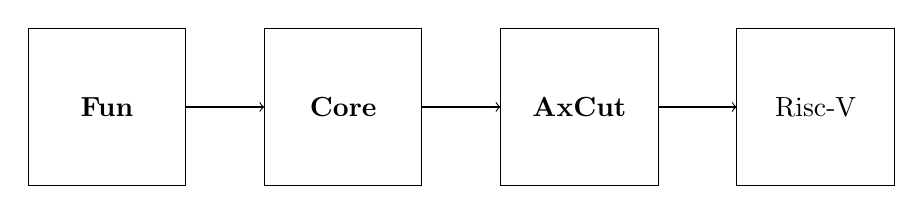
\begin{tikzpicture}
    \draw (0,0) rectangle (2,2) node[pos=.5] {\surfacelang};
    \draw (3,0) rectangle (5,2) node[pos=.5] {\targetlang};
    \draw (6,0) rectangle (8,2) node[pos=.5] {\machinelang};
    \draw (9,0) rectangle (11,2) node[pos=.5] {Risc-V};
    \draw[->] (2,1) -- (3,1);
    \draw[->] (5,1) -- (6,1);
    \draw[->] (8,1) -- (9,1);
  \end{tikzpicture}
\end{center}

The rest of this article is structured as follows:
\begin{itemize}
    \item In \cref{sec:fun} we introduce the surface language \surfacelang.
    \item In \cref{sec:core} we introduce the intermediate language \targetlang.
    \item In \cref{sec:translation} we show how to translate programs from the surface language \surfacelang\ to the intermediate language \targetlang.
    \item In \cref{sec:naming-transformation} we show a transformation on programs in \targetlang\ which names all intermediate computations, similar to ANF or focusing transformations.
    \item In \cref{sec:redundancy-elimination} and \cref{sec:substructurality-analysis} we \ldots
    \item In \cref{sec:axcut} we introduce the low-level intermediate language \machinelang, and in \cref{sec:toaxcut} we show how to compile \targetlang\ to \machinelang.
\end{itemize}
We discuss related work in \cref{sec:related-work} and conclude in \cref{sec:conclusion}.


%%
%% Section: The Surface Language Fun
%%
\section{The Surface Language Fun}
\label{sec:fun}
\begin{definition}[Syntactic Conventions]
    We use the following metavariables for all languages:
    \[
      \begin{array}{rcll}
        K & \coloneqq & \mathtt{Nil}, \mathtt{Cons}, \mathtt{Tup} & \emph{Constructors}\\
        D & \coloneqq & \mathtt{hd}, \mathtt{tl}, \mathtt{fst}, \mathtt{snd} & \emph{Destructors}\\
        \odot  & \coloneqq & + \mid - \mid * & \emph{Arithmetic Operators}
      \end{array}
    \]
  \end{definition}
  
  \begin{definition}[Syntax of Fun]
    \[ 
      \begin{array}{r c l l}
        t & \coloneqq & x \mid \lit{n} \mid t \odot t \mid \ifz{t}{t}{t} \mid \letin{x}{t}{t} \mid f(\overline{t}; \overline{\alpha}) & \emph{Terms}\\
        & \mid & K(\overline{t}) \mid \caseof{t}{\overline{K(\overline{x}) \Rightarrow t}} \mid t.D(\overline{t}) \mid \cocase{\overline{D(\overline{x}) \Rightarrow t}} & \\
        & \mid & \lambda x.t \mid t\ t \mid \lab{\alpha}{t} \mid \goto{t}{\alpha} & \\
        \Theta & \coloneqq & \emptyset \mid \defi{f(\overline{x};\overline{\alpha})}{t}; \Theta & \emph{Programs}\\
      \end{array}
    \]
  \end{definition}

%%
%% Subsec: Typing Rules
%%
\subsection{Typing Rules}
\label{subsec:fun:typing-rules}

\begin{definition}[Types and Typing Contexts]
  \[
    \begin{array}{l c l r}
      \tau   & \Coloneqq & \tyint \mid \mathtt{List}(\tau) \mid \mathtt{Pair}(\tau,\tau) \mid \mathtt{Stream}(\tau)\ \mid\ \mathtt{LPair}(\tau,\tau) \mid \tau \to \tau & \emph{Types}\\
      \Gamma & \Coloneqq & \emptyset \mid \Gamma, x \prd \tau \mid \Gamma, \alpha \cnt \tau & \emph{Typing Contexts}
    \end{array}
  \]
\end{definition}

\begin{minipage}{\textwidth}
  \begin{minipage}{0.3\textwidth}
    \begin{prooftree}
      \AxiomC{$x \prd \tau \in \Gamma$}
      \RightLabel{\textsc{Var}}
      \UnaryInfC{$\Gamma \vdash x : \tau$}
    \end{prooftree}
  \end{minipage}
  \hfill
  \begin{minipage}{0.3\textwidth}
    \begin{prooftree}
      \AxiomC{\phantom{$x : \tau \in \Gamma$}}
      \RightLabel{\textsc{Lit}}
      \UnaryInfC{$\Gamma \vdash \lit{n}:\tyint$}
    \end{prooftree}
  \end{minipage}
  \hfill
  \begin{minipage}{0.3\textwidth}
    \begin{prooftree}
      \AxiomC{$\Gamma \vdash t_1: \tyint \quad \Gamma \vdash t_2: \tyint$}
      \RightLabel{\textsc{Op}}
      \UnaryInfC{$\Gamma \vdash t_1\odot t_2 : \tyint$}
    \end{prooftree}
  \end{minipage}
  \hfill
  \vspace{1em}

  \begin{minipage}{0.55\textwidth}
    \begin{prooftree}
      \AxiomC{$\Gamma \vdash n : \tyint$}
      \AxiomC{$\Gamma \vdash t_1 : \tau$}
      \AxiomC{$\Gamma \vdash t_2 : \tau$}
      \RightLabel{\textsc{Ifz}}
      \TrinaryInfC{$\Gamma \vdash \ifz{n}{t_1}{t_2} : \tau$}
    \end{prooftree}
  \end{minipage}
  \hfill
  \begin{minipage}{0.4\textwidth}
    \begin{prooftree}
      \AxiomC{$\Gamma \vdash t_1 : \tau_1$}
      \AxiomC{$\Gamma, x \prd \tau_1 \vdash t_2 : \tau_2$}
      \RightLabel{\textsc{Let}}
      \BinaryInfC{$\Gamma \vdash \letin{x}{t_1}{t_2} :\tau_2$}
    \end{prooftree}
  \end{minipage}
  \hfill
  \vspace{1em}

  \begin{minipage}{\textwidth}
    \begin{prooftree}
      \AxiomC{$\mathbf{def}\ f(\overline{x_i \prd \tau_i};\overline{\alpha_j\cnt\tau_j}) :\tau \in P$}
      \AxiomC{$\overline{\Gamma \vdash t_i : \tau_i}$}
      \AxiomC{$\overline{\beta_j \cnt \tau_j \in \Gamma}$}
      \RightLabel{\textsc{Call}}
      \TrinaryInfC{$\Gamma \vdash f(\overline{t_i};\overline{\beta_j}) : \tau$}
    \end{prooftree}
  \end{minipage}
  \hfill
  \vspace{1em}

  \begin{minipage}{\textwidth}
    \begin{prooftree}
      \AxiomC{$\Gamma \vdash t:\mathtt{List}(\tau^{\prime})$}
      \AxiomC{$\Gamma\vdash t_1:\tau$}
      \AxiomC{$\Gamma,y\prd\tau^{\prime},z\prd\mathtt{List}(\tau^{\prime})\vdash t_2:\tau$}
      \RightLabel{\textsc{Case-List}}
      \TrinaryInfC{$\Gamma \vdash \case{t}{\mathtt{Nil}\Rightarrow t_1,\mathtt{Cons}(y,z) \Rightarrow t_2 } : \tau$}
    \end{prooftree}
  \end{minipage}
  \hfill
  \vspace{1em}

  \begin{minipage}{0.55\textwidth}
    \begin{prooftree}
      \AxiomC{$\Gamma \vdash t_1 : \tau$}
      \AxiomC{$\Gamma \vdash t_2 : \mathtt{List}(\tau)$}
      \RightLabel{\textsc{Cons}}
      \BinaryInfC{$\Gamma \vdash \mathtt{Cons}(t_1,t_2):\mathtt{List}(\tau)$}
    \end{prooftree}
  \end{minipage}
  \hfill
  \begin{minipage}{0.4\textwidth}
    \begin{prooftree}
      \AxiomC{\phantom{$\Gamma \vdash t_1 : \tau$}}
      \RightLabel{\textsc{Nil}}
      \UnaryInfC{$\Gamma \vdash \mathtt{Nil}:\mathtt{List}(\tau)$}
    \end{prooftree}
  \end{minipage}
  \hfill
  \vspace{1em}

  \begin{minipage}{0.6\textwidth}
    \begin{prooftree}
      \AxiomC{$\Gamma \vdash t:\mathtt{Pair}(\tau_1,\tau_2) \quad \Gamma,x\prd\tau_1,y\prd\tau_2 \vdash t:\tau$}
      \RightLabel{\textsc{Case-Pair}}
      \UnaryInfC{$\Gamma\vdash \case{t}{\mathtt{Tup}(x,y) \Rightarrow t}:\tau$}
    \end{prooftree}
  \end{minipage}
  \hfill
  \begin{minipage}{0.35\textwidth}
    \begin{prooftree}
      \AxiomC{$\Gamma \vdash t_1 : \tau_1 \quad \Gamma \vdash t_2 : \tau_2$}
      \RightLabel{\textsc{Tup}}
      \UnaryInfC{$\Gamma \vdash \mathtt{Tup}(t_1,t_2) : \mathtt{Pair}(\tau_1,\tau_2)$}
    \end{prooftree}
  \end{minipage}
  \hfill
  \vspace{1em}

  \begin{minipage}{0.55\textwidth}
    \begin{prooftree}
      \AxiomC{$\Gamma\vdash t:\mathtt{Stream}(\tau)$}
      \RightLabel{\textsc{Hd}}
      \UnaryInfC{$\Gamma \vdash t.\mathtt{hd} : \tau$}
    \end{prooftree}
  \end{minipage}
  \hfill
  \begin{minipage}{0.4\textwidth}
    \begin{prooftree}
      \AxiomC{$\Gamma \vdash t:\mathtt{Stream}(\tau)$}
      \RightLabel{\textsc{Tl}}
      \UnaryInfC{$\Gamma \vdash t.\mathtt{tl} : \mathtt{Stream}(\tau)$}
    \end{prooftree}
  \end{minipage}
  \hfill
  \vspace{1em}

  \begin{minipage}{\textwidth}
    \begin{prooftree}
      \AxiomC{$\Gamma\vdash t_1:\tau$}
      \AxiomC{$\Gamma\vdash t_2:\mathtt{Stream}(\tau)$}
      \RightLabel{\textsc{Stream}}
      \BinaryInfC{$\Gamma \vdash \cocase{\mathtt{hd}\Rightarrow t_1, \mathtt{tl}\Rightarrow t_2} : \mathtt{Stream}(\tau)$}
    \end{prooftree}
  \end{minipage}
  \hfill
  \vspace{1em}

  \begin{minipage}{0.55\textwidth}
    \begin{prooftree}
      \AxiomC{$\Gamma\vdash t:\mathtt{LPair}(\tau_1,\tau_2)$}
      \RightLabel{\textsc{fst}}
      \UnaryInfC{$\Gamma \vdash t.\mathtt{fst} : \tau_1$}
    \end{prooftree}
  \end{minipage}
  \hfill
  \begin{minipage}{0.4\textwidth}
    \begin{prooftree}
      \AxiomC{$\Gamma \vdash t:\mathtt{LPair}(\tau_1,\tau_2)$}
      \RightLabel{\textsc{snd}}
      \UnaryInfC{$\Gamma \vdash t.\mathtt{snd} : \tau_2$}
    \end{prooftree}
  \end{minipage}
  \hfill
  \vspace{1em}

  \begin{minipage}{\textwidth}
    \begin{prooftree}
      \AxiomC{$\Gamma\vdash t_1:\tau_1$}
      \AxiomC{$\Gamma\vdash t_2:\tau_2$}
      \RightLabel{\textsc{LPair}}
      \BinaryInfC{$\Gamma \vdash \cocase{\mathtt{fst}\Rightarrow t_1, \mathtt{snd}\Rightarrow t_2} : \mathtt{LPair}(\tau_1,\tau_2)$}
    \end{prooftree}
  \end{minipage}
  \hfill
  \vspace{1em}
 
  \begin{minipage}{0.55\textwidth}
    \begin{prooftree}
      \AxiomC{$\Gamma \vdash t_1 : \tau_1 \rightarrow \tau_2 \quad \Gamma \vdash t_2 : \tau_1$}
      \RightLabel{\textsc{App}}
      \UnaryInfC{$\Gamma \vdash t_1\ t_2 : \tau_2$}
    \end{prooftree}
  \end{minipage}
  \hfill
  \begin{minipage}{0.4\textwidth}
    \begin{prooftree}
      \AxiomC{$\Gamma,x\prd\tau_1 \vdash t:\tau_2$}
      \RightLabel{\textsc{Lam}}
      \UnaryInfC{$\Gamma \vdash \lambda x.t : \tau_1 \rightarrow \tau_2$}
    \end{prooftree}
  \end{minipage}
  \hfill
  \vspace{1em}

  \begin{minipage}{0.55\textwidth}
    \begin{prooftree}
      \AxiomC{$\Gamma \vdash t : \tau$}
      \AxiomC{$\alpha \cnt \tau \in \Gamma$}
      \RightLabel{\textsc{Goto}}
      \BinaryInfC{$\Gamma \vdash \goto{t}{\alpha} : \tau'$}
    \end{prooftree}
  \end{minipage}
  \begin{minipage}{0.4\textwidth}
    \begin{prooftree}
      \AxiomC{$\Gamma, \alpha \cnt \tau \vdash t : \tau$}
      \RightLabel{\textsc{Label}}
      \UnaryInfC{$\Gamma \vdash \lab{\alpha}{t} : \tau$}
    \end{prooftree}
  \end{minipage}
\end{minipage}
\hfill\\



%%
%% Section: The Intermediate Language Core
%%
\section{The Intermediate Language Core}
\label{sec:core}
\begin{definition}[Syntax of \targetlang{}]
  \[
    \begin{array}{rcll}
      p & \coloneqq & x \mid \lit{n} \mid \mu\alpha.s \mid K\ \sigma \mid \cocase{\overline{D\ \Gamma \Rightarrow s}} & \emph{Producers}\\
      c & \coloneqq & \alpha \mid \tilde{\mu}x.s \mid D\ \sigma \mid \case{\overline{K\ \Gamma \Rightarrow s}}& \emph{Consumers}\\
      s & \coloneqq & \cut{p}{c} \mid \ifz{p}{s}{s} \mid \odot(p, p; c) \mid f\ \sigma\mid \done & \emph{Statements}\\
      \grey{\sigma} & \grey{\coloneqq} & \grey{\nil \mid \sigma, p \mid \sigma, c} & \emph{Substitutions}\\
      \grey{\tau} & \grey{\coloneqq} & \grey{\tyint \mid T} & \emph{Types}\\
      \grey{\kappa} & \grey{\coloneqq} & \grey{\mathbf{data}\mid\mathbf{codata}\mid\mathbf{prim}} & \emph{Kinds}\\
      \grey{\Gamma} & \grey{\coloneqq} & \grey{\emptyset \mid \Gamma, x : \tau \mid \Gamma, \alpha \cnt \tau} & \emph{Typing Contexts} \\
      \delta & \coloneqq & \grey{\mathbf{data}\ T\ \{ \overline{K\ \Gamma} \}} \mid \mathbf{codata}\ T\ \{ \overline{D\ \Gamma }\} \mid \defi{f\ \Gamma}{s} & \emph{Declarations}\\
      \grey{\Theta} & \grey{\coloneqq} & \grey{\overline{\delta}} & \emph{Programs}\\
    \end{array}
  \]
\end{definition}
The most important difference between the language Fun and the language \targetlang{} are the different syntactic categories.
While Fun only had terms, \targetlang{} has producers, consumers and statements. 
As a simple approximation, terms in Fun correspond to producers in \targetlang{}, consumers correspond to continuations and statements correspond to computations. 
In \cref{sec:translation} we will explain this in more detail.

%%
%% Subsec: Typing Rules
%%
\subsection{Typing Rules}
\label{subsec:core:typing-rules}

As before, there are a number of judgements used to type expressions in \targetlang{}. 
Most of them are analogous to Fun, but since we now have producers, consumers and statements instead of terms, the typing judgement for terms has been split into three different ones. 

\begin{figure}
  \begin{minipage}{\textwidth}
    \vspace{1em}
    \judgementbox{Typing Producers}{$\Theta\mid\Gamma\vdash p:\tau$}
    \vspace{1em}
    \hfill
    \begin{minipage}{0.45\textwidth}
      \begin{prooftree}
        \AxiomC{$\Theta\mid\Gamma,\alpha\cnt \tau \vdash s$}
        \RightLabel{\textsc{$\mu$}}
        \UnaryInfC{$\Theta\mid\Gamma \vdash \mu\alpha.s:\tau$}
      \end{prooftree}
    \end{minipage}
    \hfill
    \vspace{1em}
    \begin{minipage}{0.45\textwidth}
      \begin{prooftree}
        \AxiomC{$\mathbf{codata}\ T\ \{\overline{D_i\ \Gamma_i} \}\in\Gamma$}
        \AxiomC{$\overline{\Theta\mid\Gamma,\Gamma_i \vdash s_i}$}
        \RightLabel{\textsc{Cocase}}
        \BinaryInfC{$\Theta\mid\Gamma \vdash \mathbf{cocase}\ \{\overline{D_i\ \Gamma_i\Rightarrow s_i}\} : T $}
      \end{prooftree}
    \end{minipage}
    \hfill
    \vspace{1em}
    \center{The rules \textsc{Var}, \textsc{Constructor} and \textsc{Lit} are identical to the ones in \cref{fig:fun-rules}.}
    \vspace{1em}
  \end{minipage}

  \begin{minipage}{\textwidth}
    \judgementbox{Typing Consumers}{$\Theta\mid\Gamma\vdash c\cnt \tau$}

    \begin{minipage}{\textwidth}
      \begin{prooftree}
        \AxiomC{$\Theta\mid\Gamma,x:\tau \vdash s$}
        \RightLabel{\textsc{$\tilde{\mu}$}}
        \UnaryInfC{$\Theta\mid\Gamma \vdash \tilde{\mu}x.s \cnt \tau$}
      \end{prooftree}
    \end{minipage}
    \hfill
    \vspace{1em}

    \begin{minipage}{0.45\textwidth}
      \begin{prooftree}
        \AxiomC{$\mathbf{codata}\ \{D\ \Gamma^{\prime}, \dots\}\in\Gamma$}
        \AxiomC{$\Theta\mid\Gamma \vdash \sigma:\Gamma^{\prime}$}
        \RightLabel{\textsc{Destructor}}
        \BinaryInfC{$\Theta\mid\Gamma \vdash D\ \sigma \cnt T$}
      \end{prooftree}
    \end{minipage}
    \hfill
    \begin{minipage}{0.45\textwidth}
      \begin{prooftree}
        \AxiomC{$\mathbf{data}\ \{\overline{K_i\ \Gamma_i}\}\in\Gamma$}
        \AxiomC{$\overline{\Theta\mid\Gamma,\Gamma_i\vdash s_i}$}
        \RightLabel{\textsc{Case}}
        \BinaryInfC{$\Theta\mid\Gamma \vdash \mathbf{case}\ \{ \overline{K_i\ \Gamma_i\Rightarrow s_i}\}  \cnt T$}
      \end{prooftree}
    \end{minipage}
    \hfill
    \vspace{1em}
    \center{The rule \textsc{Var}$_2$ is identical to the one in \cref{fig:fun-rules}}
    \vspace{1em}
  \end{minipage}

  \begin{minipage}{\textwidth}
    \judgementbox{Well-Typed Statements}{$\Theta\mid\Gamma \vdash s$}

    \begin{minipage}{0.3\textwidth}
      \begin{prooftree}
        \AxiomC{$\Theta\mid\Gamma \vdash p :\tau$}
        \AxiomC{$\Theta\mid\Gamma \vdash c \cnt \tau$}
        \RightLabel{\textsc{Cut}}
        \BinaryInfC{$\Theta\mid\Gamma \vdash \cut{p}{c}$}
      \end{prooftree}
    \end{minipage}
    \hfill
    \begin{minipage}{0.4\textwidth}
      \begin{prooftree}
        \AxiomC{$\Theta\mid\Gamma \vdash p : \tyint$}
        \AxiomC{$\Theta\mid\Gamma \vdash s_1$}
        \AxiomC{$\Theta\mid\Gamma \vdash s_2$}
        \RightLabel{\textsc{IfZ}}
        \TrinaryInfC{$\Theta\mid\Gamma \vdash \ifz{p}{s_1}{s_2}$}
      \end{prooftree}
    \end{minipage}
    \hfill
    \begin{minipage}{0.2\textwidth}
      \begin{prooftree}
        \AxiomC{\phantom{nothing}}
        \RightLabel{\textsc{Done}}
        \UnaryInfC{$\nil\mid\Gamma \vdash\mathbf{done}$}
      \end{prooftree}
    \end{minipage}
    \hfill
    \vspace{1em}

    \begin{minipage}{0.6\textwidth}
      \begin{prooftree}
        \AxiomC{$\Theta\mid\Gamma \vdash p_1 : \tyint$}
        \AxiomC{$\Theta\mid\Gamma \vdash p_2 : \tyint$}
        \AxiomC{$\Theta\mid\Gamma \vdash c \cnt \tyint$}
        \RightLabel{\textsc{binop}}
        \TrinaryInfC{$\Theta\mid\Gamma \vdash \odot(p_1,p_2;c)$}
      \end{prooftree}
    \end{minipage}
    \hfill
    \begin{minipage}{0.3\textwidth}
      \begin{prooftree}
        \AxiomC{$\mathbf{def}\ f\ \Gamma^{\prime} \in \Theta$}
        \AxiomC{$\Theta\mid\Gamma \vdash \sigma : \Gamma^{\prime}$}
        \RightLabel{\textsc{Call}}
        \BinaryInfC{$\Theta\mid\Gamma \vdash f\ \sigma$}
      \end{prooftree}
    \end{minipage}
    \hfill
    \vspace{1em}
  \end{minipage}

  \begin{minipage}{\textwidth}
    \judgementbox{Well-formed Programs}{$\vdash \wellformed{\Theta}$}
 
    \begin{minipage}{0.55\textwidth}
      \begin{prooftree}
        \AxiomC{$\vdash \wellformed{\Theta}$}
        \AxiomC{$\overline{\Theta,\mathbf{codata}\ T\ \{\dots\} \vdash\goodctx{\Gamma_i}}$}
        \RightLabel{\textsc{Wf-Codata}}
        \BinaryInfC{$\vdash \wellformed{\Theta,\mathbf{codata}\ T\ \{ \overline{D_i\ \Gamma_i}\}}$}
      \end{prooftree}
    \end{minipage}
    \hfill
    \begin{minipage}{0.4\textwidth}
      \begin{prooftree}
        \AxiomC{$\vdash \wellformed{\Theta}$}
        \AxiomC{$\Theta,\mathbf{def}\ f\ \Gamma \coloneq s\mid\Gamma \vdash s$}
        \RightLabel{\textsc{Wf-Fun}}
        \BinaryInfC{$\vdash \wellformed{\Theta,\mathbf{def}\ \text{f}\ \Gamma \coloneq s}$}
      \end{prooftree}
    \end{minipage}
    \hfill
    \vspace{1em}
    \center{The rules \textsc{Wf-Data} and \textsc{Wf-Empty} are identical to the ones in \cref{fig:fun-rules}}
    \vspace{1em}
  \end{minipage}
  \begin{minipage}{\textwidth}
    \fbox{\begin{minipage}{0.3\textwidth}
      \makebox[\textwidth][c]{$\Theta\mid\Gamma\vdash \sigma:\Gamma^{\prime}$ identical to \cref{fig:fun-rules}}
    \end{minipage}}
    \hfill
    \fbox{\begin{minipage}{0.3\textwidth}
      \makebox[\textwidth][c]{$\Theta\mid\Gamma\vdash \tau:\kappa$ identical to \cref{fig:fun-rules}}
    \end{minipage}}
    \hfill
    \fbox{\begin{minipage}{0.3\textwidth}
      \makebox[\textwidth][c]{{$\Theta\vdash \goodctx{\Gamma}$ identical to \cref{fig:fun-rules}}}
    \end{minipage}}
  \end{minipage}
  \caption{Typing Rules for \targetlang{}}
\end{figure}


%%
%% Section: Translation
%%
\section{Translating Fun to Core}
\label{sec:translation}
In this section we show how to translate terms of the surface language \surfacelang{} to producers of the intermediate language \targetlang.
We first introduce a simpler translation $\translate{\cdot}$ in \cref{subsec:translation:naive} which is straightforward but introduces administrative redexes.
We then introduce the optimized translation $\translatestar{\cdot}{}$ in \cref{subsec:translation:optimized} whis is more complicated, but which does not generate 
any additional administrative redexes.
We finish in \cref{subsec:translation:properties} by proving some core properties of these translation functions.

\[
  \begin{array}{rcll}
    \translate{\mathbf{codata}\ T \{ \overline{D_i\ \Gamma_i} : \tau \}}{} & \coloneq & \mathbf{codata}\ T \{ \overline{D_i\ \Gamma_i,\alpha\cnt\tau}\} & \fresh{\alpha}\\
  \end{array}
\]

Translating Declarations and typing contexts are the same for both translations we will introduce. 
Here, the most important part of the translation is the fact that codata declarations no longer have a type $\tau$ used for destructor terms.
Instead, each destructor gets a fresh covariable argument $\alpha$ with this type.
As we will see in the translations for cocases, this will ensure types are preserved under translation.

%%
%% Subsection: Naive Translation
%%
\subsection{Naive Translation}
\label{subsec:translation:naive}

First, we will introduce the naive translation, turning terms in \surfacelang{} into producers in \targetlang{}. 
As we can see from the definitions of \targetlang{} (\cref{sec:core}), certain terms, for example cases and destructors, are consumers in \targetlang{}, and others, such as if zero and top-level calls are statements.
In order to correctly translate such terms to \targetlang{}, we thus introduce $\mu$-abstractions, turning statements into producers.
Where \targetlang{}-expressions are consumers, they are cut with some other producer to turn them into statements which then make a producer with the $\mu$-abstraction.
We assume that each covariable $\alpha$ appearing in a translated term is fresh with respect to the term that is translated.
For example, when translating a top-level call $f(\overline{t_i};\overline{\alpha_i})$, the $\alpha_j$ used in the translation does not appear free in any of the $t_i$ and is not equal to any of the $\alpha_j$.
\[
  \begin{array}{rcl rcl}
    \multicolumn{6}{c}{\translate{\cdot} : \emph{Term} \rightarrow \emph{Producer}}\\
    \\
    \translate{\lit{x}} & \coloneq & \lit{x} & 
    \translate{\ifz{t_1}{t_2}{t_3}} & \coloneq & \mu\alpha.\ifz{\translate{t_1}}{\cut{\translate{t_2}}{\alpha}}{\cut{\translate{t_3}}{\alpha}} \\
    \translate{\lit{n}} & \coloneq & \lit{n}  &  
    \translate{t_1 \odot t_2} & \coloneq & \mu\alpha.\odot(\translate{t_1}, \translate{t_2}; \alpha)  \\
    \translate{f(\overline{t_i}; \overline{\alpha_j})} & \coloneq & \mu\alpha.f(\overline{\translate{t_i}}; \overline{\alpha_j},\alpha)  & 
    \translate{\letin{x}{t_1}{t_2}} & \coloneq & \mu\alpha.\cut{\translate{t_1}}{\tilde{\mu}x.\cut{\translate{t_2}}{\alpha}} \\
    \translate{K(\overline{t_i})} & \coloneq & K(\overline{\translate{t_i}}) &  
    \translate{\caseof{t}{\overline{K_i(\overline{x_{i,j}}) \Rightarrow t_i}}} & \coloneq & \mu\alpha.\cut{\translate{t}}{\case{\overline{K_i(\overline{x_{i,j}}) \Rightarrow \cut{\translate{t_i}}{\alpha}}}}  \\
    \translate{t.D(\overline{t_i})} & \coloneq & \mu\alpha.\cut{\translate{t}}{D(\overline{\translate{t_i}}; \alpha)}   & 
    \translate{\cocase{\overline{D_i(\overline{x_{ij}})\Rightarrow t_i}}} & \coloneq & \cocase{\overline{D_i(\overline{x_{i,j}}; \alpha_i) \Rightarrow \cut{\translate{t_i}}{\alpha_i}}}  \\
    \translate{\lab{\alpha}{t}} & \coloneq & \mu\alpha.\cut{\translate{t}}{\alpha} & 
    \translate{\goto{t}{\alpha}} & \coloneq & \mu\beta.\cut{\translate{t}}{\alpha}  \\
    \\
    \multicolumn{6}{c}{\translate{\cdot{}}{} : \emph{Definition}_{Fun} \rightarrow \emph{Definition}_{Core}}\\
    \multicolumn{2}{r}{\translate{\defi{f(\overline{x}; \overline{\alpha})}{t}}{}} & \multicolumn{2}{c}{\coloneq} & \multicolumn{2}{l}{\defi{f(\overline{x}; \overline{\alpha}, \alpha)}{\cut{\translate{t}}{\alpha}}} \\
    \\
  \end{array}
\]
In order to see why this translation is inefficient, consider the following term and its translation.
\begin{example}[Naive Translation of Let Bindings]
  \label{ex:translation_naive}
  \begin{align*}
    \translate{\letin{x}{\lit{2}}{x*x}} = \mu\alpha.\cut{\lit{2}}{\tilde\mu x.\cut{\mu\beta.*(x,x;\beta)}{\alpha}}
  \end{align*}
  Here, the statement bound by $\tilde\mu$ is the cut $\cut{\mu\beta.*(x,x;\beta)}{\alpha}$, which after a single reduction step becomes $*(x,x;\alpha)$.
\end{example}
Thus, whenever we introduce a new $\mu$-abstraction while translating a term in \surfacelang{}, there is a potential administrative redex generated  depending on the surrounding terms.
With these redexes included, we have two options on how to continue compilation. 
Either we keep them in the expressions and finally translate them into machine code, or we add an additional simplification step before we translate \targetlang{} to AxCut.
In each case, we will incur a performance overhead which we would like to avoid. 
To solve this issue, we will introduce the optimized translation, which keeps track of introduced covariables and only generate new ones where necessary.


%%
%% Subsection: Optimized Translation
%%
\subsection{Optimized Translation}
\label{subsec:translation:optimized}
We now introduce the optimized version of the translation introduced above.
This optimization works by splitting the function $\translate{\cdot}$ into the two functions $\translatestar{\cdot}{}$ and $\translatestar{\cdot}{k}$.
The intuition is that $\translatestar{p}{k}$ should be the same as $\cut{\translate{p}}{k}$, but whenever this results in a redex, for example if $\translate{p}$ has the form $\mu \alpha.s$, we reduce this administrative redex during the translation itself.
As before, we will again assume that any covariable $\alpha$ in the translation of a term is fresh with respect to the term being translated.

\[
  \begin{array}{rcl rcl}
    \multicolumn{6}{c}{\translatestar{\cdot}{} : \emph{Term} \rightarrow  \emph{Producer}}\\
    \translatestar{x}{} & \coloneqq & x & 
    \translatestar{\cocase{\overline{D_i(\overline{x_{i,j}}) \Rightarrow t_i}}}{} & \coloneq & \cocase{\overline{D_i(\overline{x_{i,j}}; \alpha_i) \Rightarrow \translatestar{t_i}{\alpha_i}}} \\
    \translatestar{\lit{n}}{} & \coloneqq & \lit{n}  &
    \translatestar{\lambda x.t}{} & \coloneq & \cocase{\mathtt{ap}(x; \alpha) \Rightarrow \translatestar{t}{\alpha}} \\
    \translatestar{K(\overline{t_i})}{} & \coloneqq & K(\overline{\translatestar{t_i}{}}) &
    \translatestar{\lab{\alpha}{t}}{} & \coloneq & \mu \alpha.\translatestar{t}{\alpha}{} \\
    \translatestar{t}{} & \coloneqq & \mu\alpha.\translatestar{t}{\alpha} & \fresh{\alpha} &
    \\
    \multicolumn{6}{c}{\translatestar{\cdot}{\cdot} : \emph{Term} \times \emph{Consumer} \rightarrow \emph{Statement}}\\
    \translatestar{x}{c} & \coloneq & \cut{x}{c} & 
    \translatestar{t_1 \odot t_2}{c} & \coloneq & \odot(\translatestar{t_1}{}, \translatestar{t_2}{}; c)  \\
    \translatestar{\lit{n}}{c} & \coloneq & \cut{\lit{n}}{c} & 
    \translatestar{\ifz{t_1}{t_2}{t_2}}{c} & \coloneq & \ifz{\translatestar{t_1}{}}{\translatestar{t_2}{c}}{\translatestar{t_3}{c}}  \\
    \translatestar{\letin{x}{t_1}{t_2}}{c} & \coloneq & \translatestar{t_1}{\tilde{\mu}x.\translatestar{t_2}{c}} & 
    \translatestar{f(\overline{t_i}; \overline{\alpha_j})}{c} & \coloneq & f(\overline{\translatestar{t_i}{}}; \overline{\alpha_j}, c) \\
    \translatestar{K(\overline{t_i})}{c} & \coloneq & \cut{K(\overline{\translatestar{t_i}{}})}{c} & 
    \translatestar{\caseof{t}{\overline{K_i(\overline{x_{i,j}}) \Rightarrow t_i}}}{c} & \coloneq & \translatestar{t}{\case{\overline{K_i(\overline{x_{i,j}}) \Rightarrow \translatestar{t_i}{c}}}} \\
    \translatestar{t.D(\overline{t_i})}{c} & \coloneq & \translatestar{t}{D(\overline{\translatestar{t_i}{}}; c)} &
    \translatestar{\cocase{\overline{D_i(\overline{x_{i,j}}) \Rightarrow t_i}}}{c} & \coloneq & \cut{\cocase{\overline{D_i(\overline{x_{i,j}}; \alpha_i) \Rightarrow \translatestar{t_i}{\alpha_i}}}}{c}  \\
    \translatestar{\lab{\alpha}{t}}{c} & \coloneq & \cut{\mu \alpha.\translatestar{t}{\alpha}}{c} & 
    \translatestar{\goto{t}{\alpha}}{c} & \coloneq & \translatestar{t}{\alpha} \\
    \\
    \multicolumn{6}{c}{\translatestar{\cdot}{} : \emph{Definition} \rightarrow \emph{Definition}}\\
    \multicolumn{2}{r}{\translatestar{\defi{f(\overline{x}; \overline{\alpha})}{t}}{}} & \multicolumn{2}{c}{\coloneq} & \multicolumn{2}{l}{\defi{f(\overline{x}; \overline{\alpha}, \alpha)}{\translatestar{t}{\alpha}}} 
  \end{array}
\]
To see how this translation removes administrative redexes, consider again the example \cref{example:translation:naive}
\begin{example}[Optimized Translation of Let Bindings]
  \begin{align*}
    \translate{\letin{x}{\lit{2}}{x*x}}^* = \mu\alpha.\cut{\lit{2}}{\tilde\mu x.*(x,x;\alpha)}
  \end{align*}
  The resulting producer in \targetlang{} is exactly the same as the one generated from the naive translation after reducing the administrative redex.
\end{example}
As we will see below (\cref{teo:correctness}), this property holds in general.

%%
%% Section Properties
%%
\subsection{Properties}
\label{subsec:translation:properties}

\begin{lemma}
  If $\Gamma \vdash t : \tau$ and $\Gamma' \vdash k \cnt \tau$, then $\Gamma' \vdash \translatestar{t}{k}$.
\end{lemma}
\begin{proof}
  TODO: Figure out correct statement w.r.t. $\Gamma$ and $\Gamma'$.
\end{proof}

\begin{theorem}[Type Preservation]
  Let $t$ be a term in \surfacelang, and let $\tau$ be a type.
  If $\Gamma \vdash t: \tau$, then both $\Gamma \vdash \translate{t} \prd \tau$ and $\Gamma \vdash \translatestar{t}{} \prd \tau$.
\end{theorem}

\begin{theorem}[Correctness]
  \label{teo:correctness}
  Let $t$ be a term in \surfacelang. Then there are a finite number of reduction steps (where reduction here also means reduction under binders) such that $\focus{\translate{t}} \reducesto^{\ast} \focus{\translatestar{t}{}}$, where $\focus{\cdot}$ is the focusing translation.
\end{theorem}


%%
%% Section: Naming Transformation
%%
\section{Naming Transformation}
\label{sec:naming-transformation}
We now start transforming terms of the language \targetlang{} into a normal form suitable for compilation to machine code.
The first step is to give names to all subterms.
This is a generalization of the focusing transformation which usually only names non-value producers of data types and non-value consumers of codata types.
The transformation targets the following fragment \targetvar{} of \targetlang{} where arguments of constructors, destructors and calls to top-level definitions as well as the producer arguments of conditionals and binary operators are always (co-)variables.

\begin{definition}[Syntax of \targetvar{}]
  \[
    \begin{array}{rcll}
      p & \coloneqq & x \mid \lit{n} \mid \mu\alpha.s \mid K\ \Gamma \mid \cocase{\overline{D\ \Gamma \Rightarrow s}} & \emph{Producers}\\
      c & \coloneqq & \alpha \mid \tilde{\mu}x.s \mid D\ \Gamma \mid \case{\overline{K\ \Gamma \Rightarrow s}}& \emph{Consumers}\\
      s & \coloneqq & \cut{p}{c} \mid \ifz{x}{s}{s} \mid \odot(x, x; \alpha) \mid f\ \Gamma \mid \done & \emph{Statements}\\
    \end{array}
  \]
\end{definition}

This means that substitutions now always consist of (co-)variables which is indicated in the syntax by replacing $\sigma$ by $\Gamma$.
For the corresponding typing rules we thus obtain

\vspace{1em}
\begin{minipage}{0.45\textwidth}
\begin{prooftree}
  \AxiomC{$\Theta \mid \Gamma \vdash \sigma : \Gamma^{\prime}$}
  \AxiomC{$x : \tau \in \Gamma$}
  \RightLabel{\textsc{Var}}
  \UnaryInfC{$\Theta \mid \Gamma \vdash x : \tau$}
  \RightLabel{\textsc{Subst}$_2$}
  \BinaryInfC{$\Theta \mid \Gamma \vdash \sigma, x : \Gamma^{\prime}, x : \tau$}
\end{prooftree}
\end{minipage}
\begin{minipage}{0.45\textwidth}
\begin{prooftree}
  \AxiomC{$\Theta \mid \Gamma \vdash \sigma : \Gamma^{\prime}$}
  \AxiomC{$\alpha \cnt \tau \in \Gamma$}
  \RightLabel{\textsc{Var}$_2$}
  \UnaryInfC{$\Theta \mid \Gamma \vdash \alpha \cnt \tau$}
  \RightLabel{\textsc{Subst}$_3$}
  \BinaryInfC{$\Theta \mid \Gamma \vdash \sigma, \alpha : \Gamma^{\prime}, \alpha \cnt \tau$}
\end{prooftree}
\end{minipage}
\vspace{1em}

\noindent The typing judgment for substitutions hence always becomes $\Theta \mid \Gamma \vdash \Gamma^{\prime} : \Gamma^{\prime}$ which we can abbreviate to $\Theta \mid \Gamma \vdash \Gamma^{\prime}$ with the meaning that for each $v :^{p} \tau \in \Gamma^{\prime}$ we have $v :^{p} \tau \in \Gamma$.

To make the transformation uniform, compositional and to avoid administrative redexes, it is split into three mutually recursive functions $\name{\cdot}$, $\bind{\cdot}{\cdot}$ and $\binds{\cdot}{\cdot}$, where the latter two both take a continuation as an additional argument.
The interesting part for $\name{\cdot}$ is its definition on statements for the cases where producers and consumers occur in argument positions
Therefore, the cases for a cut including a constructor or destructor are special-cased.
All other parts of $\name{\cdot}$ are simple congruences.
Types do not need to be transformed.
The idea is to lift all non-(co-)variable producers and consumers in argument positions by calling $\bind{\cdot}{\cdot}$ --- or $\binds{\cdot}{\cdot}$ in the case where a whole list of arguments is to be lifted --- and pass the statement itself in a continuation which binds fresh names for the arguments.
The function $\binds{\cdot}{\cdot}$ simply maps $\bind{\cdot}{\cdot}$ over a list of arguments, but in continuation-passing style.
The function $\bind{\cdot}{\cdot}$ pattern-matches on a given producer or consumer, transforms it recursively, creates a fresh (co-)variable and uses a $\mu$- or $\tilde\mu$-binding to bind the transformed term in a cut.
The body of the $\mu$- or $\tilde\mu$-binding consists of the given continuation applied to the freshly generated (co-)variable.
In the case where the producer or consumer is a (co-)variable already, the continuation is simply applied to it.
In the case where the producer or consumer is another constructor or destructor, the function $\binds{\cdot}{\cdot}$ is applied recursively to again lift the corresponding arguments.
Otherwise, the function $\name{\cdot}$ is recursively applied to all substatements.

\[
  \begin{array}{rclrcl}
    \\
    \multicolumn{3}{c}{\name{\cdot} : \emph{Statement}_{\targetlang{}} \rightarrow \emph{Statement}_{\targetvar{}}} &
    \multicolumn{3}{c}{\name{\cdot} : \emph{Definition}_{\targetlang{}} \rightarrow \emph{Definition}_{\targetvar{}}} \\
    \name{\cut{K\ \sigma}{c}} & \coloneq & \binds{\sigma}{\lambda as.\cut{K(as)}{\name{c}}} &
    \name{\defi{f\ \Gamma}{s}} & \coloneq & \defi{f\ \Gamma}{\name{s}} \\
    \name{\cut{p}{D\ \sigma}} & \coloneq & \binds{\sigma}{\lambda as.\cut{\name{p}}{D(as)}} \\
    \name{\cut{p}{c}} & \coloneq & \cut{\name{p}}{\name{c}} \\
    \name{\odot(p_1, p_2; c)}{} & \coloneq & \bind{p_1}{\lambda a_1.\bind{p_2}{\lambda a_2.\odot(a_1, a_2; c)}} \\
    \name{\ifz{p}{s_1}{s_2}}{} & \coloneq & \bind{p}{\lambda a.\ifz{a}{\name{s_1}}{\name{s_2}}} \\
    \name{f\ \sigma}{} & \coloneq & \binds{\sigma}{\lambda as.f(as)} \\
    \name{\done}{} & \coloneq & \done \\
    \\
    \multicolumn{3}{c}{\name{\cdot} : \emph{Producer}_{\targetlang{}} \rightarrow \emph{Producer}_{\targetvar{}}} &
    \multicolumn{3}{c}{\name{\cdot} : \emph{Consumer}_{\targetlang{}} \rightarrow \emph{Consumer}_{\targetvar{}}} \\
    \name{x} & \coloneq & x &
    \name{\alpha} & \coloneq & \alpha \\
    \name{\lit{n}} & \coloneq & \lit{n} & & & \\
    \name{\mu\alpha.s} & \coloneq & \mu\alpha.\name{s} &
    \name{\tilde{\mu}x.s} & \coloneq & \tilde{\mu}x.\name{s} \\
    \name{K\ \sigma} & \coloneq & \text{does not occur} &
    \name{D\ \sigma} & \coloneq & \text{does not occur} \\
    \name{\cocase{\overline{D_i\ \Gamma_i \Rightarrow s_i}}} & \coloneq & \cocase{\overline{D_i\ \Gamma_i \Rightarrow \name{s_i}}} &
    \name{\case{\overline{K_i\ \Gamma_i \Rightarrow s_i}}} & \coloneq & \case{\overline{K_i\ \Gamma_i \Rightarrow \name{s_i}}} \\
    \\
  \end{array}
\]

\[
  \begin{array}{rcll}
    \multicolumn{4}{c}{\bind{\cdot}{\cdot} : \emph{Producer}_{\targetlang{}} \times (\emph{Name} \rightarrow \emph{Statement}_{\targetvar{}}) \rightarrow \emph{Statement}_{\targetvar{}}}\\
    \bind{x}{k} & \coloneq & k(x) & \\
    \bind{\lit{n}}{k} & \coloneq & \cut{\lit{n}}{\tilde{\mu}x.k(x)} & \fresh{x} \\
    \bind{\mu\alpha.s}{k} & \coloneq & \cut{\mu\alpha.\name{s}}{\tilde{\mu}x.k(x)} & \fresh{x} \\
    \bind{K\ \sigma}{k} & \coloneq & \binds{\sigma}{\lambda as.\cut{K(as)}{\tilde{\mu}x.k(x)}} & \fresh{x} \\
    \bind{\cocase{\overline{D_i\ \Gamma_i \Rightarrow s_i}}}{k} & \coloneq & \cut{\cocase{\overline{D_i\ \Gamma_i \Rightarrow \name{s_i}}}}{\tilde{\mu}x.k(x)} & \fresh{x} \\
    \\
    \multicolumn{4}{c}{\bind{\cdot}{\cdot} : \emph{Consumer}_{\targetlang{}} \times (\emph{Name} \rightarrow \emph{Statement}_{\targetvar{}}) \rightarrow \emph{Statement}_{\targetvar{}}}\\
    \bind{\alpha}{k} & \coloneq & k(\alpha) & \\
    \bind{\tilde{\mu}x.s}{k} & \coloneq & \cut{\mu\alpha.k(\alpha)}{\tilde{\mu}x.\name{s}} & \fresh{\alpha} \\
    \bind{D\ \sigma}{k} & \coloneq & \binds{\sigma}{\lambda as.\cut{\mu\alpha.k(\alpha)}{D(as)}} & \fresh{\alpha} \\
    \bind{\case{\overline{K_i\ \Gamma_i \Rightarrow s_i}}}{k} & \coloneq & \cut{\mu\alpha.k(\alpha)}{\case{\overline{K_i\ \Gamma_i \Rightarrow \name{s_i}}}} & \fresh{\alpha} \\
    \\
    \multicolumn{4}{c}{\binds{\cdot}{\cdot} : \emph{Substitution} \times (\emph{List Name} \rightarrow \emph{Statement}_{\targetvar{}}) \rightarrow \emph{Statement}_{\targetvar{}}}\\
    \binds{\nil}{k} & \coloneq & k(\nil) & \\
    \binds{e :: \sigma}{k} & \coloneq & \bind{e}{\lambda a.\binds{\sigma}{\lambda as.k(a :: as)}} & \\
  \end{array}
\]


%%
%% Section: Redundancy Elimination
%%
\section{Redundancy Elimination}
\label{sec:redundancy-elimination}
The next step towards our normal consists of removing redundant part of the language.
More precisely, note that the fragment \targetvar{} explained in the previous section could as well be described with only statements, by inlining the producers and consumers into the cut statement and the consumers into the arithmetic operators.
This is because all producer and consumer arguments are (co-)variables in this fragment.
For arithmetic operators, typing only allows the consumer to be a covariable or a $\tilde\mu$-binding.
For cuts, we could in principle have 20 different forms of cuts since we have five different kinds of producers and four different kinds of consumers.
However, typing again precludes four of them: a constructor and a destructor as well as a pattern match and a copattern match can never meet in a cut, and moreover, an integer literal can never be cut with a destructor or a pattern match.
Together with conditionals, calls of top-level definitions and the terminating statement, this results in 21 statement forms in total.

We will now transform away eight of them, resulting in the following fragment \targetred{} of \targetlang{}.

\begin{definition}[Syntax of \targetred{}]
  \[
    \begin{array}{rcll}
      s & \coloneqq & \cut{K\ \Gamma}{\tilde{\mu}x.s} \mid \cut{x}{\case{\overline{K\ \Gamma \Rightarrow s}}} \mid \cut{\cocase{\overline{D\ \Gamma \Rightarrow s}}}{\tilde{\mu}x.s} \mid \cut{x}{D\ \Gamma} & \emph{Statements}\\
       & \mid & \cut{\mu\alpha.s}{D\ \Gamma} \mid \cut{\cocase{\overline{D\ \Gamma \Rightarrow s}}}{\alpha} \mid \cut{\mu\alpha.s}{\case{\overline{K\ \Gamma \Rightarrow s}}} \mid \cut{K\ \Gamma}{\alpha} & \\
       & \mid & \cut{\lit{n}}{\tilde{\mu}x.s} \mid \ifz{x}{s}{s} \mid \odot(x, x; \tilde{\mu}x.s) \mid f\ \Gamma \mid \done & \\
    \end{array}
  \]
\end{definition}

We consider the interesting cases in turn.
Let us start with the cases where a variable or covariable meets a $\tilde\mu$- or $\mu$-binding in a cut.
This is a simple renaming which we can transform away by reducing the cut via substitution.
Next, consider the cases of completely known cuts, i.e., cuts where one side is a constructor or destructor and the other side is a pattern match or copattern match.
These cuts can also simply be reduced.
As the arguments of constructors and destructors are all (co-)variables, this just amounts to picking the corresponding branch and renaming the bound (co-)variables.
Hence, there is no risk of non-termination.
Now, consider the case where a $\mu$- and a $\tilde\mu$-binding are cut, the famous critial pairs \cite{Curien2000duality}.
To transform those away, we distinguish between the different kinds of types.
For data and codata types, we have ensured that all $\eta$-laws hold by using call-by-value evaluation for data types and call-by-name evaluation for codata types.
Therefore, we can $\eta$-expand the $\tilde\mu$-binding in critical pairs of data types and the $\mu$-binding in critical pairs of data types.
For the primitive type $\tyint$, we cannot use $\eta$-expansion, so we need another way to resolve critical pairs.
The $\tilde\mu$-binding can be viewed as a continuation for integers.
As we use call-by-value evaluation for integers, we should find a different possibility to model this continuation, in such a way that the $\mu$-binding would be reduced first.
To do so, we can define a new data type:

\[
  \data{\mathtt{Cont}}{\mathtt{Ret(x : \tyint)}}
\]

\noindent A pattern match of this data type can also be viewed as a continuation for integers, the only difference from the $\tilde\mu$-binding being that the integer is wrapped into the constructor $\mathtt{Ret}$.
This means that in all places where an integer is cut with a covariable, which now stands for a consumer of type $\mathtt{Cont}$ instead of a $\tilde\mu$-binding of type $\tyint$, we have to wrap the integer into a $\mathtt{Ret}$.
There are three cases where this happens: in a cut of a variable and a covariable of type $\tyint$, in the cut of an integer literal with a covariable and in the case where the consumer of an arithmetic operator is a covariable.
For the latter two cases, we further insert a $\tilde\mu$-binding to give the integer literal or the result of the arithmetic operator a name before wrapping this name into a $\mathtt{Ret}$ which is then cut with the covariable.
It will become clear later, that no integer is ever actually wrapped into a constructor in the sense of storing it on the heap.
This is because those wrapped integers only appear in cuts with covariables in which the role of the constructor is to pick a branch in the pattern match.
As there is always only one branch, there is no overhead in modelling continuations for integers this way.
Finally, we transform away completely unknown cuts, that is, cuts of a variable with a covariable.
We have already seen above how to do this for primitive integers.
For data types and codata types we can again use $\eta$-expansion as in the cases of critical pairs, i.e., we $\eta$-expand the covariable in cuts at data types and we $\eta$-expand the variable in cuts at codata types.
All other cases are simple congruences.

\begin{gather*}
  \begin{array}{rcl}
    \multicolumn{3}{c}{\redundancy{\cdot} : \emph{Definition}_{\targetvar{}} \rightarrow \emph{Definition}_{\targetred{}}}\\
    \redundancy{\defi{f\ \Gamma}{s}} & \coloneq & \defi{f\ \Gamma}{\redundancy{s}} \\
  \end{array}
  \\\\
  \begin{array}{rclrcl}
    \multicolumn{6}{c}{\redundancy{\cdot} : \emph{Statement}_{\targetvar{}} \rightarrow \emph{Statement}_{\targetred{}}}\\
    \redundancy{\cut{\mu\alpha.s}{\beta}} & \coloneq & \redundancy{s[\alpha \mapsto \beta]} &
    \redundancy{\cut{K_j\ \Gamma_0}{\case{\overline{K_i\ \Gamma_i \Rightarrow s_i}}}} & \coloneq & \redundancy{s_j[\Gamma_j \mapsto \Gamma_0]} \\
    \redundancy{\cut{y}{\tilde{\mu}x.s}} & \coloneq & \redundancy{s[x \mapsto y]} & \qquad
    \redundancy{\cut{\cocase{\overline{D_i\ \Gamma_i \Rightarrow s_i}}}{D_j\ \Gamma_0}} & \coloneq & \redundancy{s_j[\Gamma_j \mapsto \Gamma_0]} \\
  \end{array}
  \\
  \begin{array}{rcl}
    \redundancy{\cut{\mu\alpha.s_1}{\tilde{\mu}x.s_2}_T} & \coloneq & \cut{\mu\alpha.\redundancy{s_1}}{\case{\overline{K_i\ \Gamma_i \Rightarrow \cut{K_i\ \Gamma_i}{\tilde{\mu}x.\redundancy{s_2}}}}} \\
    \text{where} &  & \data{T}{\overline{K_i\ \Gamma_i}} \in \Theta \quad \fresh{\overline{\Gamma_i}} \\
    \redundancy{\cut{\mu\alpha.s_1}{\tilde{\mu}x.s_2}_T} & \coloneq & \cut{\cocase{\overline{D_i\ \Gamma_i \Rightarrow \cut{\mu\alpha.\redundancy{s_1}}{D_i\ \Gamma_i}}}}{\tilde{\mu}x.s_2} \\
    \text{where} &  & \codata{T}{\overline{D_i\ \Gamma_i}} \in \Theta \quad \fresh{\overline{\Gamma_i}} \\
    \redundancy{\cut{\mu\alpha.s_1}{\tilde{\mu}x.s_2}_\tyint} & \coloneq & \cut{\mu\alpha.s_1}{\case{\mathtt{Ret}(x) \Rightarrow \redundancy{s_2}}} \\
    \text{where} & & \data{\mathtt{Cont}}{\mathtt{Ret(x : \tyint)}} \in \Theta \\
    \redundancy{\cut{x}{\alpha}_T} & \coloneq & \cut{x}{\case{\overline{K_i\ \Gamma_i \Rightarrow \cut{K_i\ \Gamma_i}{\alpha}}}} \\
    \text{where} &  & \data{T}{\overline{K_i\ \Gamma_i}} \in \Theta \quad \fresh{\overline{\Gamma_i}} \\
    \redundancy{\cut{x}{\alpha}_T} & \coloneq & \cut{\cocase{\overline{D_i\ \Gamma_i \Rightarrow \cut{x}{D_i\ \Gamma_i}}}}{\alpha} \\
    \text{where} &  & \codata{T}{\overline{D_i\ \Gamma_i}} \in \Theta \quad \fresh{\overline{\Gamma_i}} \\
    \redundancy{\cut{x}{\alpha}_\tyint} & \coloneq & \cut{\mathtt{Ret}(x)}{\alpha} \\
  \end{array}
  \\
  \begin{array}{rclrcl}
    \redundancy{\cut{\lit{n}}{\alpha}} & \coloneq & \cut{\lit{n}}{\tilde{\mu}x.\cut{\mathtt{Ret}(x)}{\alpha}} &
    \redundancy{\odot(x_1, x_2; \alpha)}{} & \coloneq & \odot(x_1, x_2; \tilde{\mu}x.\cut{\mathtt{Ret}(x)}{\alpha}) \\
    \text{where} &  & \fresh{x} &
    \text{where} &  & \fresh{x} \\
    \redundancy{\cut{\lit{n}}{\tilde{\mu}x.s}} & \coloneq & \cut{\lit{n}}{\tilde{\mu}x.\redundancy{s}} &
    \redundancy{\odot(x_1, x_2; \tilde{\mu}x.s)}{} & \coloneq & \odot(x_1, x_2; \tilde{\mu}x.\redundancy{s}) \\
    \redundancy{\cut{K\ \Gamma_0}{\tilde{\mu}x.s}} & \coloneq & \cut{K\ \Gamma_0}{\tilde{\mu}x.\redundancy{s}} &
    \redundancy{\cut{x}{\case{\overline{K_i\ \Gamma_i \Rightarrow s_i}}}} & \coloneq & \cut{x}{\case{\overline{K_i\ \Gamma_i \Rightarrow \redundancy{s_i}}}} \\
    \redundancy{\cut{\mu\alpha.s}{D\ \Gamma_0}} & \coloneq & \cut{\mu\alpha.\redundancy{s}}{D\ \Gamma_0} &
    \redundancy{\cut{\cocase{\overline{D_i\ \Gamma_i \Rightarrow s_i}}}{\alpha}} & \coloneq & \cut{\cocase{\overline{D_i\ \Gamma_i \Rightarrow \redundancy{s_i}}}}{\alpha} \\
    \redundancy{\cut{x}{D\ \Gamma_0}} & \coloneq & \cut{x}{D\ \Gamma_0} &
    \redundancy{\cut{\cocase{\overline{D_i\ \Gamma_i \Rightarrow s_i}}}{\tilde{\mu}x.s}} & \coloneq & \cut{\cocase{\overline{D_i\ \Gamma_i \Rightarrow \redundancy{s_i}}}}{\tilde{\mu}x.\redundancy{s}} \\
    \redundancy{\cut{K\ \Gamma_0}{\alpha}} & \coloneq & \cut{K\ \Gamma_0}{\alpha} &
    \redundancy{\cut{\mu\alpha.s}{\case{\overline{K_i\ \Gamma_i \Rightarrow s_i}}}} & \coloneq & \cut{\mu\alpha.\redundancy{s}}{\case{\overline{K_i\ \Gamma_i \Rightarrow \redundancy{s_i}}}} \\
    \redundancy{f\ \Gamma_0}{} & \coloneq & f\ \Gamma_0 &
    \redundancy{\ifz{x}{s_1}{s_2}}{} & \coloneq & \ifz{x}{\redundancy{s_1}}{\redundancy{s_2}} \\
    \redundancy{\done}{} & \coloneq & \done & & & \\
  \end{array}
\end{gather*}


%%
%% Section: AxCut
%%
\section{The Language AxCut}
\label{sec:axcut}
The astute reader may have noticed that the language \targetlang{}, and all the fragments and variations derived so far, exhibit a perfect symmetry for data and codata types and producers and consumers.
More precisely, producers of data (constructors) are perfectly symmetric to consumers of codata (destructors) and consumers of data (pattern matches) are perfectly symmetric to producers of codata (copattern matches).
We therefore can collapse the system along one of the axes shown in Figure \cref{fig:redundancy}.
Collapsing along the horizontal chirality axis means unifying producers and consumers, while collapsing along the vertical polarity axis means unifying data and codata types.
It seems more intuitive to collapse along the polarity axis, which still makes a producer and a consumer of the same type meet in a cut, resulting in a one-sided sequent calculus \cite{Girard1987}.

\begin{figure}[h!]
\tikzstyle{textonly}=[align=center, minimum width = 1.5cm, font=\small\sffamily]
\tikzstyle{box}=[textonly, rectangle, draw=black, minimum height = 1cm]
\tikzstyle{label}=[text=gray, align=center, font=\footnotesize\sffamily]

\begin{tikzpicture}[node distance=6cm, font=\footnotesize, scale=0.85, every node/.style={transform shape}]
  % Nodes
  \node (prddat) [box] at (0,0) {producer of data\\(constructor)};
  \node (cnsdat) [box] at (0,-4) {consumer of data\\(pattern match)};
  \node (prdcod) [box] at (8,0) {producer of codata\\(copattern match)};
  \node (cnscod) [box] at (8,-4) {consumer of codata\\(destructor)};

  % Arrows
  \draw [<->, >=stealth, line width = 1pt] (prddat) -- node[label, midway, above=0.1](dualtrivial){dual} (cnscod);
  \draw [<->, >=stealth, line width = 1pt] (cnsdat) -- node[label, midway, below=0.1](dualserious){dual} (prdcod);

  % Axes
  \draw [thick, dashed] (4,0.7) -- node[label, at start, right=0.1](pol){polarity} (4,-4.7);
  \draw [thick, dashed] (-1.5,-2) -- node[label, at end, above=0.1](chi){chirality} (9.5,-2);
\end{tikzpicture}

\noindent\caption{Redundancy in sequent calculus.}
\label{fig:redundancy}
\end{figure}

We use the following unified syntax for the resulting language called \machinelang, with a keyword-based syntax to make the rest of the paper more approachable to compiler engineers.

\begin{definition}[Syntax of AxCut]
    \[ 
      \begin{array}{r c l l}
        s & \coloneqq & \jump{f} \mid \substituteac{\Gamma \mapsto \Gamma}{s} \mid \done \mid \litac{n}{v}{s} \mid \opac{v, v}{v}{s} \mid \ifzac{v}{s}{s} & \emph{Statements}\\
        & \mid & \letac{v}{m\ \Gamma}{s} \mid \switch{v}{b} \mid \new{v}{\Gamma\ b}{s} \mid \invoke{v}{m} & \\
        b & \coloneqq & \bra{\overline{m\ \Gamma}} & \emph{Branches}\\
        v & \coloneqq & x \mid \alpha \mid j \mid \ldots & \emph{Variables}\\
        \tau & \coloneqq & \tyint \mid T & \emph{Types}\\
        \kappa & \coloneqq & \mathbf{sign} \mid \mathbf{prim} & \emph{Kinds}\\
        \Gamma & \coloneqq & \emptyset \mid \Gamma, v : \tau \mid \Gamma, v \cnt \tau \mid \Gamma, v \ext \tau & \emph{Typing Contexts} \\
        \delta & \coloneqq & \sig{T}{\overline{m\ \Gamma \Rightarrow s}} \mid \defi{f : \Gamma}{s} & \emph{Declarations}\\
        \Theta & \coloneqq & \overline{\delta} & \emph{Programs}\\
      \end{array}
    \]
\end{definition}

Here, $m$ is a unified notation for constructors $K$ and destructors $D$, and similarly $v$ stands for variables and covariables.
There are a few more differences to \targetsub.
We now use the $\jump{}$ construct instead of a call syntax for top-level definitions and we leave the arguments out in the syntax since they must constitute exactly the current environment.
Similarly, we leave the arguments out in the $\mathbf{invoke}$ statement where a producer $m$ is cut with a variable $v$ since the arguments of $m$ must constitute exactly the environment without $v$.
On the type level, we uniformly describe both data and codata types by signatures, without polarities, and call their unified kind $\mathbf{sign}$.
With this unification, a producer of a signature now represents a constructor or destructor and a consumer now represents a pattern match or copattern match.
We can choose to view a signature as a data type or a codata type.
We further introduce a separate typing judgment for primitive types, $\ext$, to distinguish them from producers of signatures.
Finally, we want to mention that we could make the terminal statement, the statements for integer literals and arithmetic operators and the statement for conditionals into special cases of a more general statement for external operations, $\extern{m(\overline{v_i})}{\overline{\Gamma_j \Rightarrow s_j}}$.
It is simple to extend the language with further instantiations of this general construct.

The translation from \targetsub{} to \machinelang{} mostly consists of renaming the statements to their unified counterparts.
Note how the perfectly symmetric statements of \targetsub{} are translated to exactly the same statement in \machinelang.
The most interesting part probably is the translation of type environments, where producers of data and consumers of codata in \targetsub{} are translated to the same judgment in \machinelang{} and likewise for consumers of data and producers of codata.

\begin{gather*}
  \begin{array}{rclrcl}
    \multicolumn{6}{c}{\collapse{\cdot} : \emph{Type}_{\targetsub{}} \rightarrow \emph{Type}_{\machinelang{}}}\\
    \collapse{\data{T}{\overline{K_i\ \Gamma_i}}}{} & \coloneq & \sig{T}{\overline{K_i\ \collapse{\Gamma_i}}} &
    \collapse{\Gamma, v : T}{} & \coloneq & \collapse{\Gamma}{}, v\ \collapse{: T} \\
    \collapse{\codata{T}{\overline{D_i\ \Gamma_i}}}{} & \coloneq & \sig{T}{\overline{D_i\ \collapse{\Gamma_i}}} &
    \collapse{: \tyint} & \coloneq & \ext \tyint \\
    \collapse{: T} & \coloneq & : T &
    \collapse{\cnt T} & \coloneq & \cnt T \\
    \multicolumn{3}{c}{\text{where } T : \mathbf{data}} &
    \multicolumn{3}{c}{\text{where } T : \mathbf{data}} \\
    \collapse{\cnt T} & \coloneq & : T &
    \collapse{: T} & \coloneq & \cnt T \\
    \multicolumn{3}{c}{\text{where } T : \mathbf{codata}} &
    \multicolumn{3}{c}{\text{where } T : \mathbf{codata}} \\
  \end{array}
  \\\\
  \begin{array}{rcl}
    \multicolumn{3}{c}{\collapse{\cdot} : \emph{Definition}_{\targetsub{}} \rightarrow \emph{Definition}_{\machinelang{}}}\\
    \collapse{\defi{f\ \Gamma}{s}} & \coloneq & \defi{f : \Gamma}{\collapse{s}} \\
  \end{array}
  \\\\
  \begin{array}{rclrcl}
    \multicolumn{6}{c}{\collapse{\cdot} : \emph{Statement}_{\targetsub{}} \rightarrow \emph{Statement}_{\machinelang{}}}\\
    \collapse{\cut{K\ \Gamma_0}{\tilde{\mu}x.s}} & \coloneq & \letac{x}{K\ \Gamma_0}{\collapse{s}} & \qquad
    \collapse{\cut{K\ \Gamma_0}{\alpha}} & \coloneq & \invoke{\alpha}{K} \\
    \collapse{\cut{\mu\alpha.s}{D\ \Gamma_0}} & \coloneq & \letac{\alpha}{D\ \Gamma_0}{\collapse{s}} &
    \collapse{\cut{x}{D\ \Gamma_0}} & \coloneq & \invoke{x}{D} \\
  \end{array}
  \\
  \begin{array}{rcl}
    \collapse{\cut{x}{\case{\overline{K_i\ \Gamma_i \Rightarrow s_i}}}} & \coloneq & \switch{x}{\bra{\overline{K_i\ \Gamma_i \Rightarrow \collapse{s_i}}}} \\
    \collapse{\cut{\cocase{\overline{D_i\ \Gamma_i \Rightarrow s_i}}}{\alpha}} & \coloneq & \switch{\alpha}{\bra{\overline{D_i\ \Gamma_i \Rightarrow \collapse{s_i}}}} \\
    \collapse{\cut{\mu\alpha.s}{\case{\overline{K_i\ \Gamma_i \Rightarrow s_i}}_{\Gamma_0}}} & \coloneq & \new{\alpha}{\Gamma_0 \bra{\overline{K_i\ \Gamma_i \Rightarrow \collapse{s_i}}}}{\collapse{s}} \\
    \collapse{\cut{\cocase{\overline{D_i\ \Gamma_i \Rightarrow s_i}}_{\Gamma_0}}{\tilde{\mu}x.s}} & \coloneq & \new{x}{\Gamma_0 \bra{\overline{D_i\ \Gamma_i \Rightarrow \collapse{s_i}}}}{\collapse{s}} \\
  \end{array}
  \\
  \begin{array}{rclrcl}
    \collapse{\cut{\lit{n}}{\tilde{\mu}x.s}} & \coloneq & \litac{n}{x}{\collapse{s}} &
    \collapse{\odot(x_1, x_2; \tilde{\mu}x.s)} & \coloneq & \opac{x_1, x_2}{x}{\collapse{s}} \\
    \collapse{\ifz{x}{s_1}{s_2}} & \coloneq & \ifzac{x}{\collapse{s_1}}{\collapse{s_2}} &
    \collapse{\done} & \coloneq & \done \\
    \collapse{\substitute{\Gamma \mapsto \Gamma^{\prime}}{s}} & \coloneq & \substituteac{\Gamma \mapsto \Gamma^{\prime}}{\collapse{s}} &
    \collapse{f\ \Gamma_0} & \coloneq & \jump{f} \\
  \end{array}
\end{gather*}


%%
%% Subsec: Typing Rules
%%
\subsection{Typing Rules}
\label{subsec:axcut:typing-rules}

For completeness, \cref{fig:axcut-rules} shows the full typing rules of \machinelang.

\begin{figure}[hbtp]
  \begin{minipage}{\textwidth}
  \vspace{1em}
  \judgementbox{Typing Statements}{$\Theta\mid\Gamma\vdash s$}

  \begin{minipage}{0.45\textwidth}
    \begin{prooftree}
      \AxiomC{$\Theta \mid \Gamma, v \ext \tyint \vdash s$}
      \RightLabel{\textsc{Lit}}
      \UnaryInfC{$\Theta \mid \Gamma \vdash \litac{n}{v}{s}$}
    \end{prooftree}
  \end{minipage}
  \hfill
  \begin{minipage}{0.45\textwidth}
    \begin{prooftree}
      \AxiomC{$v_1 \ext \tyint \in \Gamma$}
      \AxiomC{$v_2 \ext \tyint \in \Gamma$}
      \AxiomC{$\Theta \mid \Gamma, v \ext \tyint \vdash s$}
      \RightLabel{\textsc{Op}}
      \TrinaryInfC{$\Theta \mid \Gamma \vdash \opac{v_1, v_2}{v}{s}$}
    \end{prooftree}
  \end{minipage}
  \hfill
  \vspace{1em}

  \begin{minipage}{0.90\textwidth}
    \begin{prooftree}
      \AxiomC{$v \ext \tyint \in \Gamma$}
      \AxiomC{$\Theta \mid \Gamma \vdash s_1$}
      \AxiomC{$\Theta \mid \Gamma \vdash s_2$}
      \RightLabel{\textsc{Ifz}}
      \TrinaryInfC{$\Theta \mid \Gamma \vdash \ifzac{v}{s_1}{s_2}$}
    \end{prooftree}
  \end{minipage}
  \hfill
  \vspace{1em}

  \begin{minipage}{0.90\textwidth}
    \begin{prooftree}
      \AxiomC{$\sig{T}{{\ldots, m\ \Gamma_0, \ldots}} \in \Theta$}
      \AxiomC{$\Theta \mid \Gamma, v : T \vdash s$}
      \RightLabel{\textsc{Let}}
      \BinaryInfC{$\Theta \mid \Gamma, \Gamma_0 \vdash \letac{v}{m\ \Gamma_0}{s}$}
    \end{prooftree}
  \end{minipage}
  \hfill
  \vspace{1em}

  \begin{minipage}{0.90\textwidth}
    \begin{prooftree}
      \AxiomC{$\sig{T}{{\overline{m_i\ \Gamma_i}}} \in \Theta$}
      \AxiomC{$\overline{\Theta \mid \Gamma_i, \Gamma_0 \vdash s_i}$}
      \AxiomC{$\Theta \mid \Gamma, v \cnt T \vdash s$}
      \RightLabel{\textsc{New}}
      \TrinaryInfC{$\Theta \mid \Gamma, \Gamma_0 \vdash \new{v}{(\Gamma_0)\bra{\overline{m_i\ \Gamma_i \Rightarrow s_i}}}{s}$}
    \end{prooftree}
  \end{minipage}
  \hfill
  \vspace{1em}

  \begin{minipage}{0.45\textwidth}
    \begin{prooftree}
      \AxiomC{$\sig{T}{\overline{m_i\ \Gamma_i}} \in \Theta$}
      \AxiomC{$\overline{\Theta \mid \Gamma, \Gamma_i \vdash s_i}$}
      \RightLabel{\textsc{Switch}}
      \BinaryInfC{$\Theta \mid \Gamma, v : T \vdash \switch{v}{\bra{\overline{m_i \Gamma_i \Rightarrow s_i}}}$}
    \end{prooftree}
  \end{minipage}
  \hfill
  \begin{minipage}{0.45\textwidth}
    \begin{prooftree}
      \AxiomC{$\sig{T}{\ldots, m\ \Gamma, \ldots} \in \Theta$}
      \RightLabel{\textsc{Invoke}}
      \UnaryInfC{$\Theta \mid \Gamma, v \cnt T \vdash \invoke{v}{m}$}
    \end{prooftree}
  \end{minipage}
  \hfill
  \vspace{1em}

  \begin{minipage}{0.22\textwidth}
    \begin{prooftree}
      \AxiomC{\phantom{nothing}}
      \RightLabel{\textsc{Done}}
      \UnaryInfC{$\Theta \mid \Gamma \vdash \done$}
    \end{prooftree}
  \end{minipage}
  \hfill
  \begin{minipage}{0.43\textwidth}
    \begin{prooftree}
      \AxiomC{$\Theta \mid v'_1 :^{p} \tau, \ldots \vdash s$}
      \AxiomC{$v_1 :^{p} \tau \in \Gamma \ldots$}
      \RightLabel{\textsc{Substitute}}
      \BinaryInfC{$\Theta \mid \Gamma \vdash \substituteac{v'_1 \mapsto v_1, \ldots}{s}$}
    \end{prooftree}
  \end{minipage}
  \hfill
  \begin{minipage}{0.25\textwidth}
    \begin{prooftree}
      \AxiomC{$\mathbf{def}\ f\ \Gamma \in \Theta$}
      \RightLabel{\textsc{Jump}}
      \UnaryInfC{$\Theta \mid \Gamma \vdash \jump{f}$}
    \end{prooftree}
  \end{minipage}
  \hfill
  \vspace{1em}
\end{minipage}
\begin{minipage}{\textwidth}
  \vspace{1em}
  \judgementbox{Kinding Types}{$\Theta\vdash\tau:\kappa$}
  \begin{minipage}{0.4\textwidth}
    \begin{prooftree}
      \AxiomC{}
      \RightLabel{\textsc{PrimKind}}
      \UnaryInfC{$\Theta \vdash \tyint : \mathbf{prim}$}
    \end{prooftree}
  \end{minipage}
  \hfill
  \begin{minipage}{0.5\textwidth}
    \begin{prooftree}
      \AxiomC{$\sig{T}{\ldots} \in \Theta$}
      \RightLabel{\textsc{SignatureKind}}
      \UnaryInfC{$\Theta \vdash T : \mathbf{sign}$}
    \end{prooftree}
  \end{minipage}
  \vspace{1em}
\end{minipage}
\begin{minipage}{\textwidth}
  \vspace{1em}
  \judgementbox{Well-formed Programs}{$\vdash \wellformed{\Theta}$}
  \begin{minipage}{0.2\textwidth}
    \begin{prooftree}
      \AxiomC{}
      \RightLabel{\textsc{Wf-Empty}}
      \UnaryInfC{$\vdash \wellformed{\nil}$}
    \end{prooftree}
  \end{minipage}
  \hfill
  \begin{minipage}{0.75\textwidth}
    \begin{prooftree}
      \AxiomC{$\vdash \wellformed{\Theta}$}
      \AxiomC{$\overline{\Theta,\sig{T}{\dots}\vdash\goodctx{\Gamma_i}}$}
      \AxiomC{$\overline{ \Gamma_i \vdash \tau_i:\kappa}$}
      \RightLabel{\textsc{Wf-Signature}}
      \TrinaryInfC{$\vdash \wellformed{\Theta,\sig{T}{ \overline{m_i\ \Gamma_i}}}$}
    \end{prooftree}
  \end{minipage}
  \hfill
  \vspace{1em}

  \begin{minipage}{0.90\textwidth}
    \begin{prooftree}
      \AxiomC{$\vdash \wellformed{\Theta}$}
      \AxiomC{$\Theta, \defi{f : \Gamma}{s} \mid\Gamma \vdash s$}
      \RightLabel{\textsc{Wf-Def}}
      \BinaryInfC{$\vdash \wellformed{\Theta,\defi{f : \Gamma}{s}}$}
    \end{prooftree}
  \end{minipage}
  \hfill
  \vspace{1em}
\end{minipage}
\begin{minipage}{\textwidth}
  \vspace{1em}
  \judgementbox{Well-formed Contexts}{$\Theta\vdash \goodctx{\Gamma}$}
  \begin{minipage}{0.45\textwidth}
    \begin{prooftree}
      \AxiomC{\phantom{$x\in\nil$}}
      \RightLabel{\textsc{Ctx}$_1$}
      \UnaryInfC{$\Theta\vdash\goodctx{\nil}$}
    \end{prooftree}
  \end{minipage}
  \hfill
  \vspace{1em}
  \begin{minipage}{0.45\textwidth}
    \begin{prooftree}
      \AxiomC{$\Theta\vdash\goodctx{\Gamma} \quad v\notin\Gamma \quad \Theta\vdash\tau:\kappa$}
      \RightLabel{\textsc{Ctx}$_2$}
      \UnaryInfC{$\Theta\vdash\goodctx{\Gamma,v:\tau}$}
    \end{prooftree}
  \end{minipage}
  \hfill
  \vspace{1em}
  \begin{minipage}{0.45\textwidth}
    \begin{prooftree}
      \AxiomC{$\Theta\vdash\goodctx{\Gamma} \quad v\notin\Gamma \quad \Theta\vdash\tau:\kappa$}
      \RightLabel{\textsc{Ctx}$_3$}
      \UnaryInfC{$\Theta\vdash \goodctx{\Gamma,v\cnt\tau}$}
    \end{prooftree}
  \end{minipage}
  \hfill
  \vspace{1em}
  \begin{minipage}{0.45\textwidth}
    \begin{prooftree}
      \AxiomC{$\Theta\vdash\goodctx{\Gamma} \quad v\notin\Gamma \quad \Theta\vdash\tau:\kappa$}
      \RightLabel{\textsc{Ctx}$_4$}
      \UnaryInfC{$\Theta\vdash \goodctx{\Gamma,v\ext\tau}$}
    \end{prooftree}
  \end{minipage}
  \hfill
  \vspace{1em}
\end{minipage}
\caption{Typing rules for \machinelang{}}
\label{fig:axcut-rules}
\end{figure}


%%
%% Section: Translation to AxCut
%%
\section{Translation to AxCut}
\label{sec:toaxcut}
This is the translation from \targetlang{} to \machinelang, assuming that the program was named and redundancy-eliminated.
It collapses data and codata types, renames constructs and inserts explicit subtitutions.
The subtitutions aim to drop unneeded variables as early as possible and duplicate variables as late as possible to reduce the register pressure.
(I'm not perfectly sure whether the insertions are fully correct (i.p., with respect to shadowing) and there may be a better solution.)

\[
  \begin{array}{rcll}
    \multicolumn{4}{c}{\axcutify{\cdot}{} : \emph{Type}_{\targetred{}} \rightarrow \emph{Type}_{\machinelang{}}}\\
    \axcutify{\data{T}{\overline{K_i\ \Gamma_i}}}{} & \coloneq & \sig{T}{\overline{K_i\ \axcutify{\Gamma_i}{}}} & \\
    \axcutify{\codata{T}{\overline{D_i\ \Gamma_i}}}{} & \coloneq & \sig{T}{\overline{D_i\ \axcutify{\Gamma_i}{}}} & \\
    \axcutify{\Gamma, v : T}{} & \coloneq & \axcutify{\Gamma}{}, v\ \axcutify{: T}{} & \\
    \axcutify{: T}{} & \coloneq & : T & \text{where } T : \mathbf{data} \\
    \axcutify{\cnt T}{} & \coloneq & \cnt T & \text{where } T : \mathbf{data} \\
    \axcutify{: T}{} & \coloneq & \cnt T & \text{where } T : \mathbf{codata} \\
    \axcutify{\cnt T}{} & \coloneq & : T & \text{where } T : \mathbf{codata} \\
    \axcutify{: \tyint}{} & \coloneq & \ext \tyint & \\
  \end{array}
\]

\[
  \begin{array}{rcll}
    \multicolumn{4}{c}{\axcutify{\cdot}{} : \emph{Definition}_{\targetred{}} \rightarrow \emph{Definition}_{\machinelang{}}}\\
    \axcutify{\defi{f(\overline{x}; \overline{\alpha})}{s}}{} & \coloneq & \defi{f(\overline{x}, \overline{\alpha})}{\substitute{\Gamma' \mapsto \Gamma'}{\axcutify{s}{\Gamma'}}} & \\
    \text{where} &  & \Gamma' = (\overline{x}, \overline{\alpha}) \cap \free{s} & \\
    \\
    \multicolumn{4}{c}{\axcutify{\cdot}{\cdot} : \emph{Statement}_{\targetred{}} \times \emph{Context}_{\machinelang{}} \rightarrow \emph{Statement}_{\machinelang{}}}\\
    \axcutify{\cut{K\ \Gamma_0}{\tilde{\mu}x.s}}{\Gamma} & \coloneq & \substitute{\Gamma' \mapsto \Gamma', \Gamma_0 \mapsto \Gamma_0}{\letac{x}{K(\Gamma_0)}{\axcutify{s}{\Gamma', x}}} & \\
    \text{where} &  & \Gamma' = (\Gamma - x) \cap \free{s} \text{ (substraction only needed if variables not unique)} & \\
    \axcutify{\cut{\mu\alpha.s}{D\ \Gamma_0}}{\Gamma} & \coloneq & \substitute{\Gamma' \mapsto \Gamma', \Gamma_0 \mapsto \Gamma_0}{\letac{\alpha}{D\ \Gamma_0}{\axcutify{s}{\Gamma', \alpha}}} & \\
    \text{where} &  & \Gamma' = (\Gamma - \alpha) \cap \free{s} & \\
    \axcutify{\cut{K\ \Gamma_0}{\alpha}}{\Gamma} & \coloneq & \substitute{\Gamma_0 \mapsto \Gamma_0, \alpha \mapsto \alpha}{\invoke{\alpha}{K}} & \\
    \axcutify{\cut{x}{D\ \Gamma_0}}{\Gamma} & \coloneq & \substitute{\Gamma_0 \mapsto \Gamma_0, x \mapsto x}{\invoke{x}{D}} & \\
    \axcutify{\cut{x}{\case{\overline{K_i\ \Gamma_i \Rightarrow s_i}}}}{\Gamma} & \coloneq & \substitute{\Gamma' \mapsto \Gamma', x \mapsto x}{\switch{x}{\bra{\overline{K_i\ \Gamma_i \Rightarrow \axcutify{s_i}{\Gamma', \Gamma_i}}}}} & \\
    \text{where} &  & \Gamma' = \Gamma \cap \bigcup_i \free{s_i} & \\
    \axcutify{\cut{\cocase{\overline{D_i\ \Gamma_i \Rightarrow s_i}}}{\alpha}}{\Gamma} & \coloneq & \substitute{\Gamma' \mapsto \Gamma', \alpha \mapsto \alpha}{\switch{\alpha}{\bra{\overline{D_i\ \Gamma_i \Rightarrow \axcutify{s_i}{\Gamma', \Gamma_i}}}}} & \\
    \text{where} &  & \Gamma' = \Gamma \cap \bigcup_i \free{s_i} & \\
    \axcutify{\cut{\mu\alpha.s}{\case{\overline{K_i\ \Gamma_i \Rightarrow s_i}}}}{\Gamma} & \coloneq & \substitute{\Gamma' \mapsto \Gamma', \Gamma_0 \mapsto \Gamma_0}{\new{\alpha}{(\Gamma_0)\bra{\overline{K_i\ \Gamma_i \Rightarrow \axcutify{s_i}{\Gamma_i, \Gamma_0}}}}{\axcutify{s}{\Gamma', \alpha}}} & \\
    \text{where} &  & \Gamma_0 = \Gamma \cap \bigcup_i \free{s_i}  \quad  \Gamma' = (\Gamma - \alpha) \cap \free{s} & \\
    \axcutify{\cut{\cocase{\overline{D_i\ \Gamma_i \Rightarrow s_i}}}{\tilde{\mu}x.s}}{\Gamma} & \coloneq & \substitute{\Gamma' \mapsto \Gamma', \Gamma_0 \mapsto \Gamma_0}{\new{x}{(\Gamma_0)\bra{\overline{D_i\ \Gamma_i \Rightarrow \axcutify{s_i}{\Gamma_i, \Gamma_0}}}}{\axcutify{s}{\Gamma', x}}} & \\
    \text{where} &  & \Gamma_0 = \Gamma \cap \bigcup_i \free{s_i}  \quad  \Gamma' = (\Gamma - x) \cap \free{s} & \\
    \axcutify{\cut{\lit{n}}{\tilde{\mu}x.s}}{\Gamma} & \coloneq & \substitute{\Gamma' \mapsto \Gamma'}{\litac{n}{x}{\axcutify{s}{\Gamma', x}}} & \\
    \text{where} &  & \Gamma' = (\Gamma - x)\cap \free{s} & \\
    \axcutify{\odot(x_1, x_2; \tilde{\mu}x.s)}{\Gamma} & \coloneq & \substitute{\Gamma' \mapsto \Gamma'}{\opac{x_1, x_2}{x}{\axcutify{s}{\Gamma', x}}} & \\
    \text{where} &  & \Gamma' = (\Gamma - x) \cap (x_1 \cup x_2 \cup \free{s}) & \\
    \axcutify{\ifz{x}{s_1}{s_2}}{\Gamma}{} & \coloneq & \ifzac{x}{\axcutify{s_1}{\Gamma}}{\axcutify{s_2}{\Gamma}} & \\
    \axcutify{f\ \Gamma_0}{\Gamma} & \coloneq & \substitute{\Gamma_0 \mapsto \Gamma_0}{\jump{f}} & \\
    \axcutify{\done}{\Gamma} & \coloneq & \done & \\
  \end{array}
\]


%%
%% Section: Related Work
%%
\section{Related Work}
\label{sec:related-work}
\begin{itemize}
    \item \cite{Downen2016sequent}
\end{itemize}


%%
%% Section: Conclusion
%%
\section{Conclusion}
\label{sec:conclusion}
\input{sections/conclusion.tex}

%%
%% Bibliography
%%
\bibliography{bibliography/bibliography.bib, bibliography/ownpublications.bib}

\end{document}
